%-------------------------
% Resume in Latex
% Author : Sourabh Bajaj
% Website: https://github.com/sb2nov/resume
% License : MIT
%------------------------
\documentclass[letterpaper,11pt]{article}

\usepackage{latexsym}
\usepackage[empty]{fullpage}
\usepackage{titlesec}
\usepackage{marvosym}
\usepackage[usenames,dvipsnames]{color}
\usepackage{verbatim}
\usepackage{enumitem}
\usepackage[pdftex]{hyperref}
\usepackage{fancyhdr}
\usepackage{graphicx} % Added for image handling

\pagestyle{fancy}
\fancyhf{} % clear all header and footer fields
\fancyfoot{}
\renewcommand{\headrulewidth}{0pt}
\renewcommand{\footrulewidth}{0pt}

% Adjust margins
\addtolength{\oddsidemargin}{-0.375in}
\addtolength{\evensidemargin}{-0.375in}
\addtolength{\textwidth}{1in}
\addtolength{\topmargin}{-.5in}
\addtolength{\textheight}{1.0in}

\urlstyle{same}

\raggedbottom
\raggedright
\setlength{\tabcolsep}{0in}

% Sections formatting
\titleformat{\section}{
	\vspace{-4pt}\scshape\raggedright\large
}{}{0em}{}[\color{black}\titlerule \vspace{-5pt}]

%-------------------------
% Custom commands
\newcommand{\resumeItem}[2]{
	\item\small{
		\textbf{#1}{: #2 \vspace{-2pt}}
	}
}

\newcommand{\resumeSubheading}[4]{
	\vspace{-1pt}\item
	\begin{tabular*}{0.97\textwidth}{l@{\extracolsep{\fill}}r}
		\textbf{#1} & #2 \\
		\textit{\small#3} & \textit{\small #4} \\
	\end{tabular*}\vspace{-5pt}
}

\newcommand{\resumeSubItem}[2]{\resumeItem{#1}{#2}\vspace{-4pt}}

\renewcommand{\labelitemii}{$\circ$}

\newcommand{\resumeSubHeadingListStart}{\begin{itemize}[leftmargin=*]}
	\newcommand{\resumeSubHeadingListEnd}{\end{itemize}}
\newcommand{\resumeItemListStart}{\begin{itemize}}
	\newcommand{\resumeItemListEnd}{\end{itemize}\vspace{-5pt}}

%-------------------------------------------
%%%%%%  CV STARTS HERE  %%%%%%%%%%%%%%%%%%%%%%%%%%%%


\begin{document}
	
	%----------HEADING-----------------
	\begin{tabular*}{\textwidth}{l@{\extracolsep{\fill}}r}
		\begin{tabular}[t]{l}
			\textbf{\href{hissamshar.github.io/}{\Large Hisam Mehboob}} \\
			\href{https://hissamshar.github.io/}{hissamshar.github.io} \\
			Email: \href{mailto:hisamshar@gmail.com}{hisamshar@gmail.com} \\
			Mobile: +92 323 3587380 \\
			Github: \href{https://github.com/hissamshar}{hissamshar}
		\end{tabular} &
		\raisebox{-0.8\totalheight}{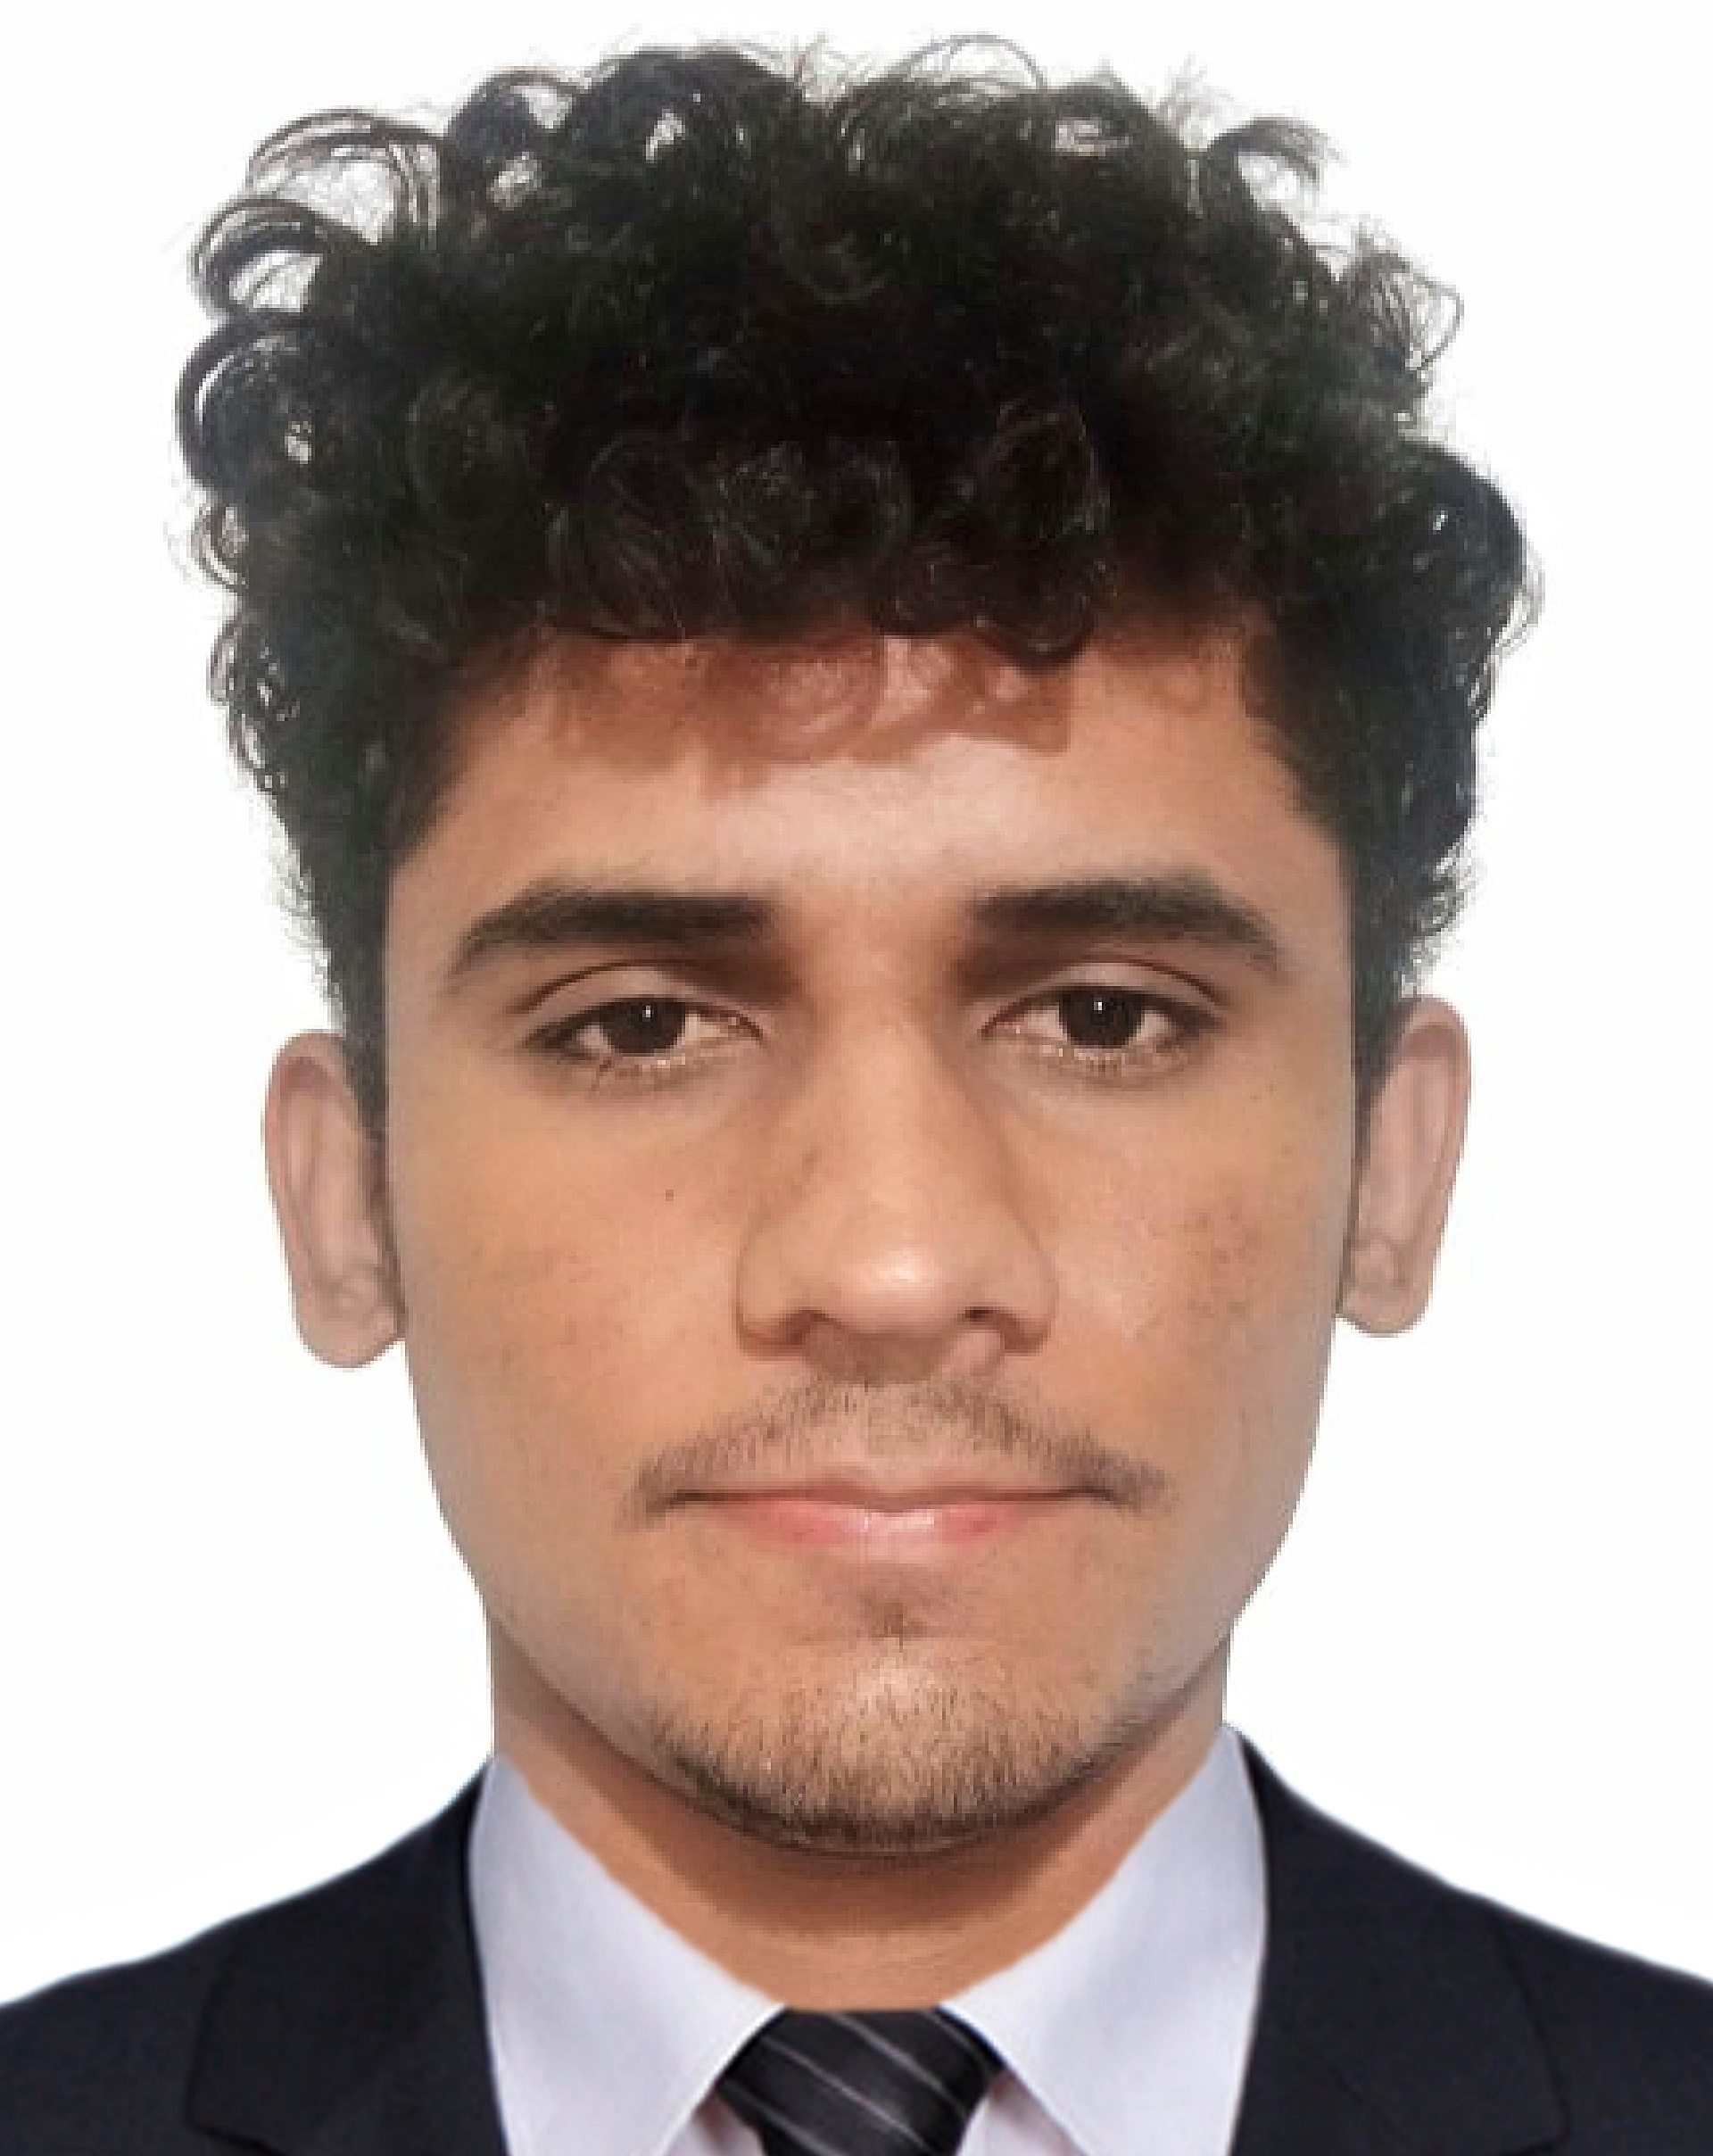
\includegraphics[width=2.4cm]{PROFILE.jpeg}} \\ % Adjust image path and size
	\end{tabular*}
	
	%--------PROGRAMMING SKILLS------------
	\section{Profile}
Computer Science student with hands-on experience in systems and embedded programming, aiming to build innovative, low-level tech solutions that bridge hardware and software.
	
	%-----------EXPERIENCE-----------------
	\section{Experience}
	\resumeSubHeadingListStart
	
	\resumeSubheading
	{COLAB NU}{Peshawar, Khyber Pakhtunkhwa}
	{Tier 1 Member}{Oct 2024 - Present}
	\resumeItemListStart
	\resumeItem{Hugo}
	{Developed static websites using Hugo, leveraging its fast build times and Go-based architecture for efficient content management and templating.}
	\resumeItem{Kernal Programming}
	{Created custom Linux kernel modules, focusing on low-level system optimization, device drivers, and hardware-software interaction for enhanced performance.}
	
	\resumeItem{Raspberry Pi 5 }
	{Engineered IoT and embedded systems solutions using Raspberry Pi 5, integrating GPIO, and hardware automation for custom projects.}
	\resumeItemListEnd
	
	%-----------PROJECTS-----------------
	%-----------PROJECTS-----------------
\section{Projects}

\resumeSubItem{Text Editor}
{Coded in C/C++ with no dependencies, and it implements all the basic features.}

\resumeSubItem{POSIX Shell}
{Built a Portable Operating System Interface compliant shell in C langauge.}

\resumeSubItem{Ray Tracing}
{Implemented a ray tracer from scratch using C++ gaining hands-on experience in rendering algorithms, 3D graphics, and computational geometry.}

\resumeSubItem{Nand2Tetris}
{Built a modern computer system from the ground up, designing hardware components (from logic gates to CPU) and software layers (assembler, virtual machine, and compiler) to create a computer capable of running high-level programs.}

%\resumeSubItem{Recommendation System}
%{Music and Movie recommender systems using collaborative filtering on public datasets.}
%     \resumeSubItem{Mac Setup}
%       {Book that gives step by step instructions on setting up developer environment on Mac OS.}
\resumeSubHeadingListEnd
	
	%-----------Communities Work:-----------------
	\section{Communities Work}
	\resumeSubHeadingListStart
	\resumeSubheading
	{IEEE FAST NUCES, Fast National University Peshawar}{\textbf{Mar. 2025 -- Present}}
	{Junior Representative}{}
	\resumeItemListStart
	\resumeItem{Work}
	{Participated in IEEE-hosted campus events, workshops, and tech seminars to expand knowledge in cutting-edge engineering trends and network with industry peers.}
	\resumeItemListEnd
	

	
	%-----------EDUCATION-----------------
	\section{Education}

\resumeSubheading
{National University of Computer and Emerging Sciences}{\textbf{Aug. 2024 -- Jun. 2028}}
{Bachelor of Science in Computer Science; CGPA:3.50}{}
\resumeItemListStart
\resumeItem{Coursework}
{Operating Systems, Parallel and Distributed Computing, Computer Organization and
	Assembly Language, Data Structures, Algorithms, Software Testing and Debugging.}
\resumeItemListEnd

\resumeSubHeadingListEnd



		%
	%--------PROGRAMMING SKILLS------------
	\section{Skills and Participations}
	\begin{itemize}[leftmargin=*]
		\item \textbf{IT Support Skills}{: Troubleshooting, MS Office, Networking Basics, Documentation, Communication}
		\item \textbf{Languages}{: C, C++, Python, Javascript, Markdown}
		\item \textbf{Technologies}{: Hugo, LaTex, RPi 5, Qemu/KVM, Git, GitHub}
		\item \textbf{Participations}{: FAST Problem-Solving Challenge, Codeforces, NaScon}
	\end{itemize}



\end{document}